\chapter{Results}\label{ch:results}
In this chapter, we will briefly describe the datasets tested and the results of our experiments.  We will then discuss our findings, looking at the confusion matrices and focusing on four metrics: Accuracy, Average Accuracy ($\overline{A}$), Matthew's Correlation Coefficient (MCC) and Confusion Entropy.  We can to MCC and CEN later in the project, but they provide some insight into multidimensional confusion matrices.  A brief introduction to the two metrics follows.\\
MCC is a real valued number between -1 and 1, and is equivalent to $$\frac{cov(X,Y)}{\sqrt{cov(X,X)\cdot cov(Y,Y)}}$$
The magnitude measures the amount of information not attributable to random chance.  A 1 is a perfect correlation with the data, only achievable when accuracy is also equal to 1.  A -1 is a perfect anti-correlation, though generating it is not as simple as merely getting everything wrong.  Finally, a 0 means that the prediction is performing no better than chance.  For further information, we recommend \cite{jurman_comparison_2012}.\\
\cite{wei_novel_2010} contains the full detail and motivation regarding CEN, which ranges from 0 to 1.  In this case, 0 indicates a perfect matrix, and 1 virtually no self-information.  To be crude but generally accurate, CEN is a measure of the probability of misclassification of classes by the classifier.  Thus, lower is better. We calculate it as\\
 \begin{align*}
CEN &= - \sum_{j}^{N+1}P_j\sum_{k}^{N+1}P^j_{j,k}log_N(P^j_{j,k}) + P^j_{k,j}log_N(P^j_{k,j})\\
\\
P^i_{i,j}&=\frac{C_{i,j}}{\sum_{k=1}^{N+1}C_{i,k} + C_{k,i}}\\
\\
P^j_{i,j}&=\frac{C_{i,j}}{\sum_{k=1}^{N+1}C_{j,k} + C_{k,j}}\\
\\
P_j&= \frac{\sum_{k=1}^{N+1}C_{j,k}+ C_{k,j}}{2\sum_{k,l}^{N+1}}C_{k,l}\\	
\end{align*}	\\Where C is the confusion matrix.  $P_j$ is the probability of misclassifying a particular class, $P^i_{i,j}$ is the probability of misclassifying $\omega_i$ as $\omega_j$ subject to class i, and $P^j_{i,j}$ is the same, but subject to class j.  To understand this, pay particular attention to the denominators where the classes sum over different "crosses", centered at the superscripted variable which is fixed, while k iterates both horizontally and vertically across the matrix.  Also, for calculation purposes, $P^i_{i,i}$ = 0, and logs of 0 in the density function may also be treated as 0.  
\section{Datasets}
All of our datasets were acquired from the UCI database \citep{lichman_uci_2013}.  We used 3 different datasets, trying to span multiple fields of study.  To that end we used Yeast \citep{paul_horton_uci_1996}, which is a relatively simple biological dataset, Cardioctocography \citep{j._p._marques_de_sa_uci_2010} (Cardio) which is a medical dataset, and Bach's Chorales \citep{daniele_p._radicioni_uci_2014} which is a musical dataset.  With minimal configuration, described in Chapter 2, our program can handle virtually any dataset in the standard matrix form.  We will first describe the makeup of the dataset, provide a visualization of the data through a method called t-distributed stochastic neighbor embedding(T-SNE) first developed in \cite{maaten_visualizing_2008}.\\
T-SNE is conceptually similar to K-Nearest Neighbors, in that it is unsupervised and assumes that things which are similar will be nearby in whatever n-dimensional space they are embedded in.  Indeed, T-SNE takes the distances of each point to all other points and converts them to probabilities, then builds probability density functions maximizing their likelihood.  The density functions in this case are student-T distributions, which are similar Gaussian distributions but their tails are much fatter- that is, they don't go to zero nearly as quickly.  Once these distributions are built T-SNE iteratively performs a form of gradient descent minimizing the error of the predictions of the T distributions.  It is very good at maintaining separability found at high dimensions into lower-dimensional spaces, which makes it good for plotting. However, there are concerns that it may not be particularly good at doing dimensional reduction, which often means a reliance on Principal Component Analysis or some similar method to handle that portion.\\
\paragraph{Yeast Dataset}
This dataset is used to predict the localizations of proteins in a yeast's cell.  Its meanings and usage are fully motivated in \cite{nakai_knowledge_1992}.  For our purposes, each sample (of 1484) belong to one of 10 classes, which correlate to their function within the cell.  The original paper used an expert system which boasted 59\% accuracy.  For a visualization of Yeast, see figure \ref{fig:yeasttsne}.  This should be the best case scenario.  There are very few features, and a handful of classes, so barring inseparable data (which the visualization demonstrates to not be the case) there should be little trouble for a classifier to find some signal in the data.


\begin{figure}
	\centering
	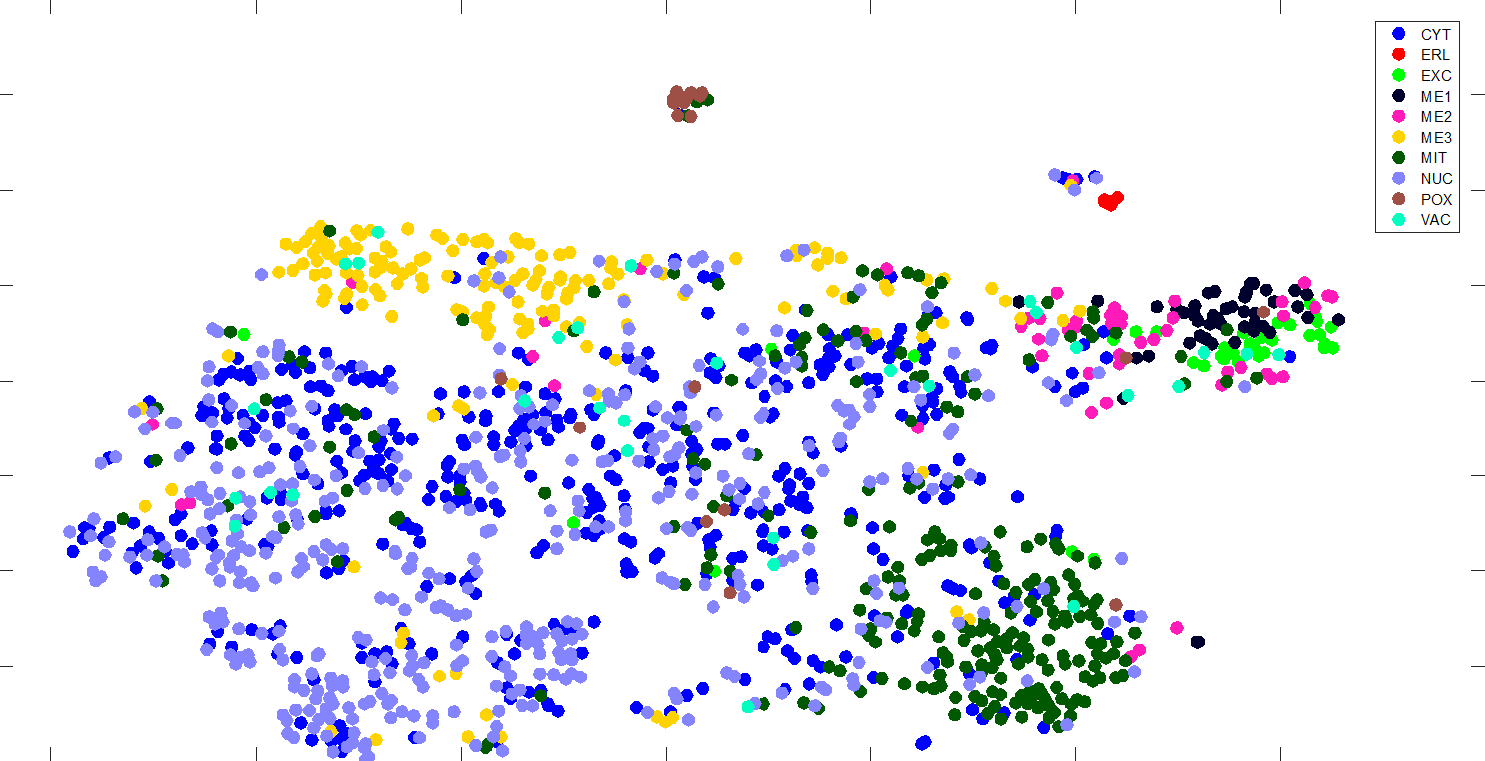
\includegraphics[width=0.9\linewidth]{figures/png/YeastTSNE}
	\caption[T-SNE visualization of Yeast dataset]{T-SNE visualization of Yeast dataset. Viewing in color is highly recommended.}
		\label{fig:yeasttsne}
\end{figure}



\paragraph{Cardiotocography Dataset}
Cardiotocography is the practice of monitoring fetal heartbeats during pregnancy.  The Cardiotocograph (CTG) is the machine used to monitor, and it produces cardiotocograms.    The dataset is based on \cite{ayres-de-campos_sisporto_2000} and was also used, in limited form, in \cite{ocak_medical_2013}, where the researchers achieved an impressive 100\% specificity (in this case, the correct classification of pathologic cardiotocograms).  Their sensitivity was also very high- 99.3\% on the training set.  Clearly here specificity is more important than sensitivity!  Unfortunately, these researchers left out approximately 200 samples of suspicious cardiotocograms, which confound things considerably.  There are good methodological reasons for doing this, of course- SVMs don't work as well with more than 2 classes, and culturally medicine is very concerned with sensitivity and specificity, which don't apply to non-binary problems in general.  We certainly aren't criticizing the good work medical researchers do, nor the lives they save.\\
We do include the suspect cardiotocograms, so we don't expect our results to be quite as clean. Further, there are two classification modes in this dataset, not 1.  The first is what we've mentioned already, the Normal, Suspect, Pathologic (NSP) classifications.  The second is the morphologic patterns 1-10.  These may or may not overlap with the NSP, but they provide a second way of looking at the data and evaluating it.  We have provided T-SNE visualizations with both colorings below in \ref{fig:cardio3tsne} and \ref{fig:cardio10tsne}.
\begin{figure}
	\centering
	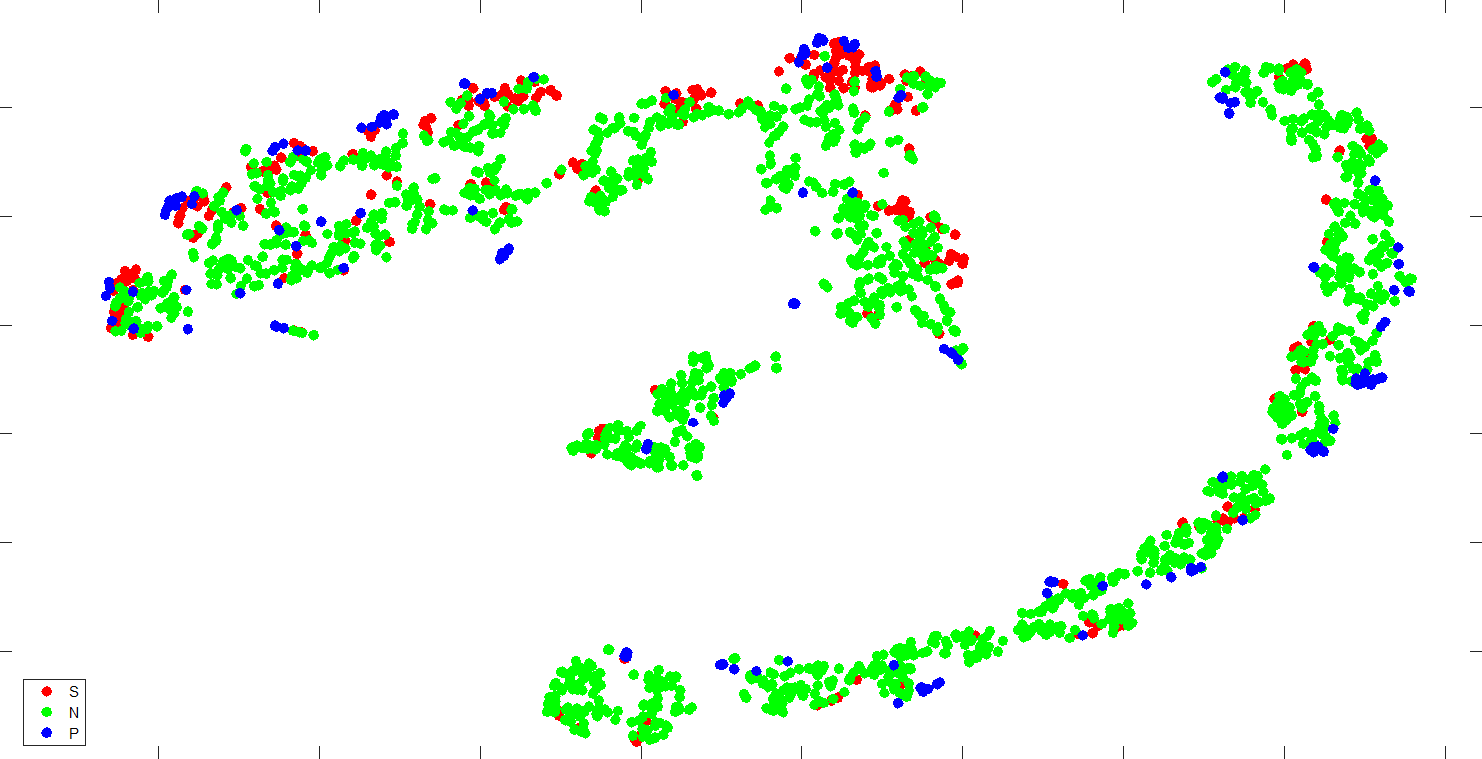
\includegraphics[width=0.9\linewidth]{figures/png/Cardio3TSNE}
	\caption[T-SNE visualization of Cardio dataset, NSP]{T-SNE visualization of Cardio dataset, following the NSP classification schema.}
	\label{fig:cardio3tsne}
\end{figure}
\begin{figure}
	\centering
	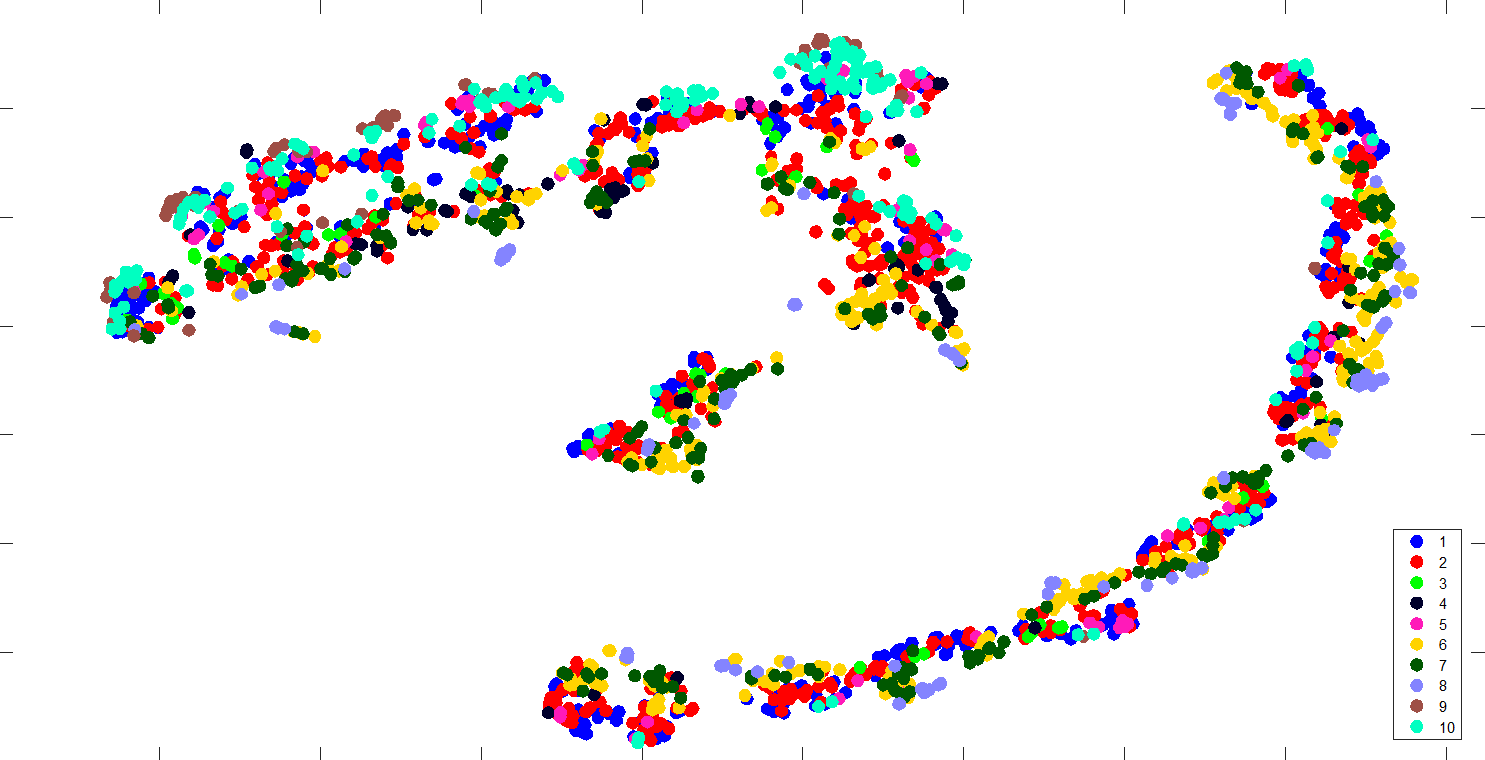
\includegraphics[width=0.9\linewidth]{figures/png/Cardio10TSNE}
	\caption[T-SNE visualization of Cardio dataset, morphology]{T-SNE visualization of Cardio dataset, following the 10-class morphology schema.  Viewing in color is highly recommended.}
	\label{fig:cardio10tsne}
\end{figure}
\paragraph{Bach's Chorales}
Bach composed all manner of music, but this dataset comprises 58 of his 4 part harmonies, called Chorales.  Originally made a dataset in \cite{radicioni_breve:_2010} the music of 58 chorales are painstakingly broken into 5665 musical moments, such that every time there are 3 or more distinct notes being played it their proper key is classified- but there are confounding factors. Primarily, there might be added notes, which means a note must always be taken in context, which makes the problem much more difficult.  What was a fairly modest 36 classes (12 notes $\times$ 3 modes) becomes 108 when added notes are taken into account.  Originally the authors used a perceptron which scored 75\% accuracy, which is certainly much better than chance because, while there are 108 possible classes, only 102 can actually be found in the dataset.  \\We should note that we modified this dataset slightly.  Initially they were published in the order in which they occurred.  We added an additional feature including the key of the previous event and then randomized the order of the file before splitting it into training and testing sets.  The hopes were that our algorithms would be able to take advantage of the temporal information in their models, even if they weren't explicitly instructed that it was temporal.  The visualization (\ref{fig:bachtsne}) is difficult to read because of the many classes, but clearly delineates several inherent clusters.
\begin{figure}
	\centering
	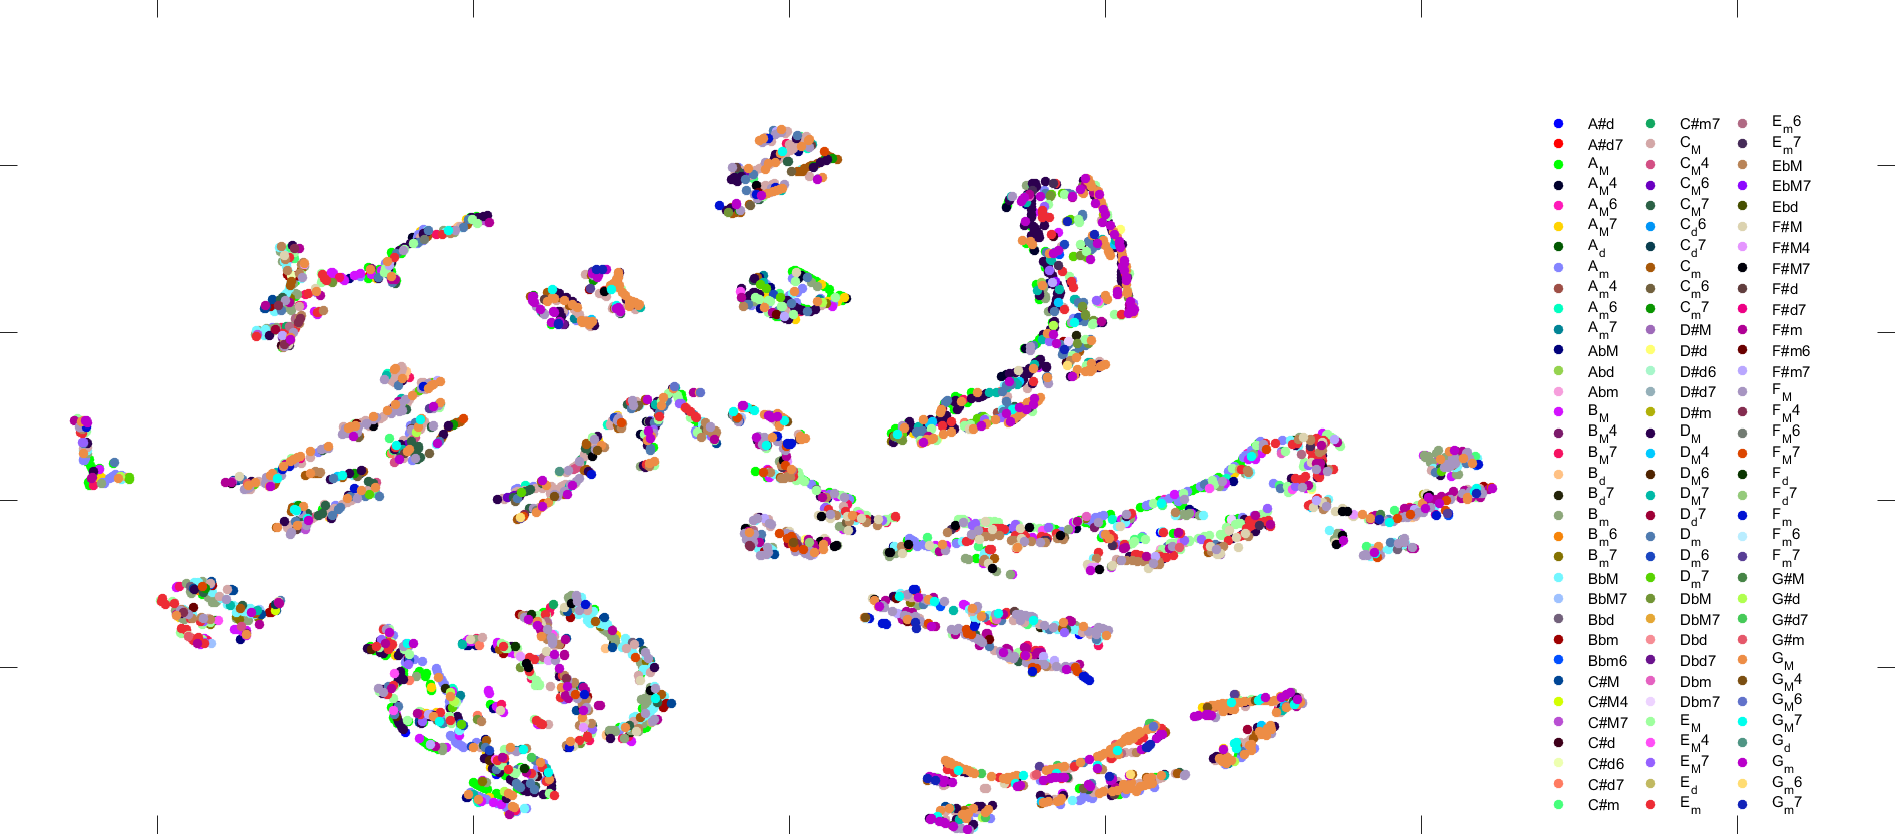
\includegraphics[width=0.9\linewidth]{figures/png/BachTSNE}
	\caption[T-SNE visualization of Bach dataset]{T-SNE visualization of 102 class Bach dataset.  Classes are incredibly difficult to distinguish, but instead focus on the overall shapes and distinct clusters.}
	\label{fig:bachtsne}
\end{figure}
\section{Results}
\subsection{Yeast}

\paragraph{CTree Baseline}:
As we can see, the baseline did fairly well regarding the 3 most common classes, but its ability to distinguish the less frequent classifications suffered giving it a final $\overline{A}$ of 64.1\%, or an overall accuracy of 74.6\%. See table \ref{tab:yeastctreebase} for more detail.\\
\begin{table}[h!]
\begin{tabular}{|c|c|c|c|c|c|c|c|c|c|c|c|}
\hline
Class&MIT&NUC&CYT&ME1&EXC&ME2&ME3&VAC&POX&ERL&Total
\\\hline
MIT&151&14&24&0&0&5&2&1&1&1&199\\
NUC&8&145&36&0&1&0&4&1&3&0&198\\
CYT&19&30&133&0&3&4&1&2&5&1&198\\
ME1&1&0&0&14&2&1&0&0&0&0&18\\
EXC&0&0&0&0&12&0&0&0&0&0&12\\
ME2&0&1&1&2&1&21&0&0&0&0&26\\
ME3&1&4&3&1&0&2&67&0&0&0&78\\
VAC&0&1&0&0&0&0&0&1&0&0&2\\
POX&0&0&1&0&0&0&0&0&5&0&6\\
ERL&0&0&0&0&0&0&0&0&0&3&3\\
\hline
Total:&180&195&198&17&19&33&74&5&14&5&740\\
TPR:&0.839&0.744&0.672&0.824&0.632&0.636&0.905&0.2&0.357&0.6&0.641\\
\hline
\end{tabular}
\caption[Yeast: Classification Tree without Feature Selection Confusion Matrix]{Yeast Dataset, Classification Tree with all features included, Accuracy = 74.6\%, MCC: 0.674 CEN: 0.273}
\label{tab:yeastctreebase}
\end{table}

\paragraph{CTree w/ feature selection}:
With feature selection $\overline{A}$ increased modestly to 65.8\%, but accuracy declined to 68.4\%.  See table \ref{tab:yeastctreefeatures}.\\  
\begin{table}[h]

\begin{tabular}{|c|c|c|c|c|c|c|c|c|c|c|c|}
	\hline
Class&MIT&NUC&CYT&ME1&EXC&ME2&ME3&VAC&POX&ERL&Total\\
MIT&131&13&9&0&0&1&2&0&2&0&158\\
NUC&8&87&26&0&1&0&1&2&0&0&125\\
CYT&33&87&158&0&3&2&4&2&4&0&293\\
ME1&1&0&0&13&2&1&0&0&0&0&17\\
EXC&1&0&0&1&11&1&0&0&0&0&14\\
ME2&5&2&1&2&2&26&0&0&0&1&39\\
ME3&1&5&3&1&0&2&67&0&0&0&79\\
VAC&0&1&0&0&0&0&0&1&0&0&2\\
POX&0&0&1&0&0&0&0&0&8&0&9\\
ERL&0&0&0&0&0&0&0&0&0&4&4\\
\hline
Total:&180&195&198&17&19&33&74&5&14&5&740\\
TPR:&0.728&0.446&0.798&0.765&0.579&0.788&0.905&0.2&0.571&0.8&0.658\\
\hline


\end{tabular}
\caption[Yeast: Classification Tree with Feature Selection Confusion Matrix]{Yeast Dataset, Classification Tree with feature selection, Accuracy = 68.4\%, MCC: 0.607 CEN: 0.290}
\label{tab:yeastctreefeatures}
\end{table}

\paragraph{McNB Baseline}
With all features, $\overline{A}$ was quite good: 85.9\%.  However, overall accuracy was 72.8\%.  See table \ref{tab:yeastctreebase} for confusion matrix and other details.
\\
\begin{table}[h!]
\begin{tabular}{|c|c|c|c|c|c|c|c|c|c|c|c|}
	\hline
Class&MIT&NUC&CYT&ME1&EXC&ME2&ME3&VAC&POX&ERL&Total\\\hline
MIT&119&10&10&0&0&0&1&0&1&0&141\\
NUC&9&108&17&0&0&1&0&0&0&0&135\\
CYT&18&35&152&0&1&0&0&1&0&0&207\\
ME1&4&4&2&17&0&0&0&0&0&0&27\\
EXC&4&6&2&0&18&0&0&0&0&0&30\\
ME2&12&9&5&0&0&32&2&0&0&0&60\\
ME3&8&10&5&0&0&0&71&0&0&0&94\\
VAC&1&5&0&0&0&0&0&4&0&0&10\\
POX&5&8&5&0&0&0&0&0&13&0&31\\
ERL&0&0&0&0&0&0&0&0&0&5&5\\
\hline
Total:&180&195&198&17&19&33&74&5&14&5&740\\
TPR:&0.661&0.554&0.768&1&0.947&0.97&0.959&0.8&0.929&1&0.859\\
\hline
\end{tabular}
\caption[Yeast: Multiclass Na\"ive Bayes without Feature Selection Confusion Matrix]{Yeast Dataset, Multiclass Na\"ive Bayes with all features included, Accuracy = 72.8\%, MCC: 0.671 CEN: 0.293}
\label{tab:yeastmcnbbase}
\end{table}

\paragraph{McNB w/ feature selection:}
With feature selection, Multiclass Na\"ive Bayes had the highest $\overline{A}$ of 87\%, though with an accuracy of only 72.8\%.  The disparity is accounted for in the accuracy across the first 3 classes, which make up more than $\frac{3}{4}$ of the dataset.  On them, accuracy ranged between abysmal and mediocre.  We can clearly see the danger of a highly skewed dataset and the dangers of metrics than are do not take this sufficiently into account.  See table \ref{tab:yeastctreebase} for details.
\\
\begin{table}[h!]
\begin{tabular}{|c|c|c|c|c|c|c|c|c|c|c|c|}
	\hline
Class&MIT&NUC&CYT&ME1&EXC&ME2&ME3&VAC&POX&ERL&Total\\
\hline
MIT&124&22&17&0&0&0&0&0&1&0&164\\
NUC&8&90&21&0&0&0&0&0&0&0&119\\
CYT&13&36&134&0&1&0&0&0&0&0&184\\
ME1&3&1&1&17&0&0&0&0&0&0&22\\
EXC&2&3&1&0&18&0&0&0&0&0&24\\
ME2&9&8&4&0&0&33&0&0&0&0&54\\
ME3&15&20&12&0&0&0&74&0&0&0&121\\
VAC&2&9&3&0&0&0&0&5&0&0&19\\
POX&4&5&5&0&0&0&0&0&13&0&27\\
ERL&0&1&0&0&0&0&0&0&0&5&6\\
\hline
Total:&180&195&198&17&19&33&74&5&14&5&740\\
TPR:&0.689&0.462&0.677&1&0.947&1&1&1&0.929&1&0.87\\
\hline
\end{tabular}
\caption[Yeast: Multiclass Na\"ive Bayes with Feature Selection Confusion Matrix]{Yeast Dataset, Multiclass Na\"ive Bayes with feature selection included, Accuracy = 72.8\%, MCC: 0.630 CEN: 0.310}
\label{tab:yeastmcnbfeatures}
\end{table}



	\paragraph{Hunter}
The Hunter underperformed the four other methods by any measure, and took a great deal (more than 100 times) more processor time to do it.  This was supposed to be the best case for the Hunters, and early indications say that it is.  $\overline{A}$ = .473\%, while accuracy is 51.1\%.  Table \ref{tab:yeasthunter}.
\\
	% TODO: Write writeup, interpret bits
\begin{table}[h!]
		\begin{tabular}{|c|c|c|c|c|c|c|c|c|c|c|c|}
		\hline
		Class&MIT&NUC&CYT&ME1&EXC&ME2&ME3&VAC&POX&ERL&Total\\
		\hline
MIT&105&17&12&0&0&0&0&0&0&0&134\\
NUC&2&37&10&1&0&1&3&0&0&0&54\\
CYT&43&94&142&0&5&3&2&1&10&0&300\\
ME1&4&1&0&8&1&3&7&0&0&0&24\\
EXC&9&2&3&0&9&7&0&0&2&0&32\\
ME2&1&9&6&6&4&12&1&1&0&2&42\\
ME3&14&5&11&2&0&6&58&1&0&0&97\\
VAC&2&28&13&0&0&1&3&2&0&0&49\\
POX&0&0&1&0&0&0&0&0&2&0&3\\
ERL&0&2&0&0&0&0&0&0&0&3&5\\
\hline
Total:&180&195&198&17&19&33&74&5&14&5&740\\
TPR:&0.583&0.19&0.717&0.471&0.474&0.364&0.784&0.4&0.143&0.6&0.473\\

		\hline
	\end{tabular}
	\caption[Yeast: Hunter]{Yeast Dataset, Hunter Accuracy = 51.1\%, MCC: 0.413 CEN: 0.409}
	\label{tab:yeasthunter}
\end{table}

Which classifier performed best is open for debate, both CTree and McNB are promising in their own ways.  CTree seems to do a better job with the bulk classes, and perhaps if you're optimizing average accuracy that's a good way to go- optimize a method for something it is less suited for, resulting in a kind of check on optimization gone awry.  Alternatively, perhaps the status of the major classes aren't as important, and the focus instead is on discriminating between the outlying classes.  In that case, McNB clearly wins.  In any case, the Hunter performed.  It didn't do well, exactly, and with more time it might have done better, but that applies to any of these methods.  The difference is that the Hunter already had 10 times as many generations and still didn't manage to get anywhere even close to competitive.

\subsection{Cardiotocography NSP}
\paragraph{CTree Baseline}
A classification tree handily gets 94\% accuracy on this dataset, but that will prove to be a fairly unsurprising given this dataset.  See table \ref{tab:cardioNSPctreebase} for more details.
\begin{table}[h!]
	\centering
	\begin{tabular}{|c|c|c|c|c|}
		\hline
		Class&Normal&Suspect&Pathologic&Total\\\hline
Normal&519&31&9&559\\
Suspect&12&408&0&420\\
Pathologic&10&0&74&84\\\hline
Total:&541&439&83&1063\\
TPR:&0.959&0.929&0.892&0.927\\
		\hline
	\end{tabular}
	\caption[Cardiotocography NSP: Classification Tree without Feature Selection Confusion Matrix]{Cardio Dataset, NSP Labels Classification Tree without feature selection included, Accuracy=94.1\%, MCC: 0.967 CEN: 0.043}
	\label{tab:cardioNSPctreebase}
\end{table}
\paragraph{CTree w/ Feature Selection}
With feature selection, we see a similar pattern to yeast.  Overall accuracy drops slightly, but the smaller classes get more accurate.  What's interesting here is that MCC and CEN both decrease; see table \ref{tab:cardioNSPctree} for more details.
\begin{table}[h]
	\centering
	\begin{tabular}{|c|c|c|c|c|}
		\hline
		Class&Normal&Suspect&Pathologic&Total\\\hline
Normal&514&34&3&551\\
Suspect&12&405&0&417\\
Pathologic&15&0&80&95\\\hline
Total:&541&439&83&1063\\
TPR:&0.95&0.923&0.964&0.946\\

		\hline
	\end{tabular}
	\caption[Cardiotocography NSP: Classification Tree with Feature Selection Confusion Matrix]{Cardio Dataset, NSP Labels Classification Tree with feature selection included, Accuracy: 93.9\% MCC: 0.962 CEN: 0.051}
	\label{tab:cardioNSPctree}
\end{table}

\paragraph{McNB Baseline}
We get an accuracy of 90.2\%, which is low compared to the previous classifiers, and the supporting metrics of MCC and CEN are much worse as well.  See table \ref{tab:cardioNSPmcnbbase} for details.
\begin{table}[h]
	\centering
	\begin{tabular}{|c|c|c|c|c|}
		\hline
Class&Normal&Suspect&Pathologic&Total\\\hline
Normal&476&24&6&506\\
Suspect&37&408&2&447\\
Pathologic&28&7&75&110\\\hline
Total:&541&439&83&1063\\
TPR:&0.88&0.929&0.904&0.904\\
\hline
	\end{tabular}
	\caption[Cardiotocography NSP: Multiclass Na\"ive Bayes without Feature Selection Confusion Matrix]{Cardio Dataset, NSP Labels Multiclass Na\"ive Bayes without feature selection included, Accuracy = 90.2\% MCC: 0.797 CEN: 0.186}
\label{tab:cardioNSPmcnbbase}
\end{table}
\paragraph{McNB w/ Feature Selection}
Here, McNB manages to redeem itself somewhat.  $\overline{A}$ is the highest for any of the classifiers, and accuracy is only slightly lower than the baseline CTree.  However, MCC and CEN are considerably worse than that tree- so take this classifiers' predictions with a grain of salt.  
\begin{table}[h]
	\centering
	\begin{tabular}{|c|c|c|c|c|}
		\hline
Class&Normal&Suspect&Pathologic&Total\\\hline
Normal&490&11&1&502\\
Suspect&28&427&0&455\\
Pathologic&23&1&82&106\\\hline
Total:&541&439&83&1063\\
TPR:&0.906&0.973&0.988&0.956\\
\hline
	\end{tabular}
	\caption[Cardiotocography NSP: Multiclass Na\"ive Bayes with Feature Selection Confusion Matrix]{Cardio Dataset, NSP Labels Multiclass Na\"ive Bayes with feature selection included, Accuracy = 94\%, MCC: 0.889 CEN: 0.116}
	\label{tab:cardioNSPmcnb}
\end{table}

\paragraph{Hunter}
This is probably the best we will see from the Hunter.  That said, it didn't do very well for the purpose of the dataset, which is distinguishing pathologic patterns from safe ones.  See table \ref{tab:cardioNSPHunter} for further discussion.

\begin{table}[h!]
	\centering
	\begin{tabular}{|c|c|c|c|c|}
		\hline
		Class&Normal&Suspect&Pathologic&Total\\\hline
Normal&197&77&10&284\\
Suspect&183&322&4&509\\
Pathologic&161&40&69&270\\\hline
Total:&541&439&83&1063\\
TPR:&0.364&0.733&0.831&0.643\\
		\hline
	\end{tabular}
	\caption[Cardiotocography NSP: Hunter Confusion Matrix]{Cardio Dataset, NSP Labels Hunter, Accuracy = 55\%, MCC: 0.333 CEN: 0.568}
	\label{tab:cardioNSPHunter}
\end{table}

As we can see, the CTree without feature selection performed best on this dataset.  For one thing, the dataset was developed by experts and they selected features that would be most indicative of problems.  Also, it might seem strange that MCC and CEN were so much lower on the Bayesian classifiers.  In examining the tables, pay close attention to how well the total in the right column matches the total in the row, and that should give an idea of why.  In some sense, MCC and CEN are measures of the useful information from the classifier.  In this case, when it makes a prediction of a particular class it's extremely confident.  That's much more useful than what the Bayesian classifiers discern, \textit{even though they get more of the pathological cases correct}.  Because even though the McNB with feature selection gets 82 of the 83 pathological cases, it also misclassified them about 20\% of the time. 
\subsection{Cardiotocography Morphology}
\paragraph{CTree Baseline}  
Again, this dataset proves to be highly separable, and CTree continues to do quite well.  See table \ref{tab:cardiomorphctreebase} for details. 
\begin{table}[h!]
	\centering
	\begin{tabular}{|c|c|c|c|c|c|c|c|c|c|c|c|}
	\hline
		Class&J&F&A&H&G&B&D&I&E&C&Total\\
\hline
		J&97&0&2&0&0&0&0&0&2&0&101\\
		F&0&159&0&1&5&6&0&0&0&0&171\\
		A&4&0&183&0&0&5&0&0&1&1&194\\
		H&0&0&0&42&2&0&1&0&0&2&47\\
		G&0&1&1&0&120&1&0&0&0&0&123\\
		B&0&0&1&0&0&286&3&0&3&1&294\\
		D&0&1&0&0&0&1&38&0&0&0&40\\
		I&3&0&1&0&0&0&0&28&0&0&32\\
		E&2&0&5&0&0&1&0&0&31&1&40\\
		C&0&0&2&0&0&0&0&0&0&19&21\\\hline
		Total:&106&161&195&43&127&300&42&28&37&24&1063\\
		TPR:&0.915&0.988&0.938&0.977&0.945&0.953&0.905&1&0.838&0.792&0.925\\
		\hline
	\end{tabular}
	\caption[Cardiotocology Morphology: Classification Tree  Confusion Matrix]{Cardio Dataset, Morphological Labels Classification Tree without feature selection included, Accuracy = 94.3\% MCC: 0.933, CEN: 0.086}
	\label{tab:cardiomorphctreebase}
\end{table}

\paragraph{CTree w/ Feature Selection}
Compared to the baseline, accuracy increased marginally but MCC got slightly worse.  CEN stayed the same to 3 significant figures.  See table \ref{tab:cardiomorphctree}.
\begin{table}
	\centering	
	\begin{tabular}{|c|c|c|c|c|c|c|c|c|c|c|c|}
	\hline
	Class&J&F&A&H&G&B&D&I&E&C&Total\\
	\hline
	J&98&0&0&0&0&0&0&0&2&1&101\\
	F&0&161&1&1&1&7&0&0&0&0&171\\
	A&6&0&178&0&0&4&0&1&3&2&194\\
	H&0&0&2&44&0&0&1&0&0&0&47\\
	G&0&4&1&0&118&0&0&0&0&0&123\\
	B&0&1&3&0&0&283&3&0&4&0&294\\
	D&0&1&0&0&0&0&39&0&0&0&40\\
	I&3&0&0&0&0&0&0&29&0&0&32\\
	E&1&0&5&0&0&0&0&0&33&1&40\\
	C&0&0&2&0&0&0&0&0&0&19&21\\\hline
	Total:&108&167&192&45&119&294&43&30&42&23&1063\\
	TPR:&0.907&0.964&0.927&0.978&0.992&0.963&0.907&0.967&0.786&0.826&0.922\\
	\hline
\end{tabular}
	\caption[Cardiotocology Morphology: Classification Tree Confusion Matrix]{Cardio Dataset, Morphological Labels Classification Tree with feature selection included accuracy: 94.3\% MCC: 0.931, CEN: 0.086}
	\label{tab:cardiomorphctree}
\end{table}
\paragraph{McNB Baseline}
Here, we again see the discriminative power of the Bayesian method- accuracy is up to 96\% and CEN is down a full 3.5 points and MCC is up by almost the same.  There's one class, I, where 100\% of the cases were caught, that is, one perfect column, though there's no corresponding perfect row.  See table \ref{tab:cardiomorphmcnbbase}.
\begin{table}[h!]
	\centering
	\begin{tabular}{|c|c|c|c|c|c|c|c|c|c|c|c|}
\hline
Class&J&F&A&H&G&B&D&I&E&C&Total\\
\hline
J&99&0&2&0&0&0&0&0&0&0&101\\
F&0&169&0&0&0&1&0&0&0&1&171\\
A&2&0&189&0&0&2&0&0&0&1&194\\
H&0&0&0&47&0&0&0&0&0&0&47\\
G&0&1&0&1&121&0&0&0&0&0&123\\
B&0&5&9&0&2&276&1&0&1&0&294\\
D&0&0&0&0&0&0&40&0&0&0&40\\
I&2&0&0&0&0&0&0&30&0&0&32\\
E&2&0&0&0&0&0&0&0&38&0&40\\
C&0&0&0&0&0&0&0&0&0&21&21\\\hline
Total:&105&175&200&48&123&279&41&30&39&23&1063\\
TPR:&0.943&0.966&0.945&0.979&0.984&0.989&0.976&1&0.974&0.913&0.967\\
\hline
	\end{tabular}
	\caption[Cardiotocography Morphology:  Na\"ive Bayes without Feature Selection Confusion Matrix]{Cardio Dataset Morphological Labels Multiclass Na\"ive Bayes without feature selection, Accuracy= 96.9\% MCC: 0.963, CEN: 0.05}
	\label{tab:cardiomorphmcnbbase}
\end{table}
\paragraph{McNB w/ Feature Selection}
This is the best we'll likely see from McNB: there are 3 perfect columns and 3 rows, and they overlap on 2 of the classes (I and H).  Accuracy and $\overline{A}$ are 98.3 and 98.1\%, respectively, MCC is 0.980 and CEN is 0.030.  See table \ref{tab:cardiomorphmcnb} for further details.
\begin{table}[h!]
	\centering
	\begin{tabular}{|c|c|c|c|c|c|c|c|c|c|c|c|}
		\hline
	Class&J&F&A&H&G&B&D&I&E&C&Total\\
	\hline
	J&100&0&1&0&0&0&0&0&0&0&101\\
	F&0&171&0&0&0&0&0&0&0&0&171\\
	A&0&0&187&0&1&4&0&0&1&1&194\\
	H&0&0&0&47&0&0&0&0&0&0&47\\
	G&0&1&0&0&122&0&0&0&0&0&123\\
	B&0&4&2&0&1&285&1&0&1&0&294\\
	D&0&0&0&0&0&0&40&0&0&0&40\\
	I&0&0&0&0&0&0&0&32&0&0&32\\
	E&0&0&0&0&0&0&0&0&40&0&40\\
	C&0&0&0&0&0&0&0&0&0&21&21\\
\hline
	Total:&100&176&190&47&124&289&41&32&42&22&1063\\
	TPR:&1&0.972&0.984&1&0.984&0.986&0.976&1&0.952&0.955&0.981\\
	
		\hline
	\end{tabular}
	\caption[Cardiotocography Morphology:  Na\"ive Bayes without Feature Selection Confusion Matrix]{Cardio Dataset Morphological Labels Multiclass Na\"ive Bayes with feature selection, Accuracy = 98.3\%, MCC: 0.98, CEN: 0.03}
	\label{tab:cardiomorphmcnb}
\end{table}
\paragraph{Hunter}
This hunter actually manages a negative MCC, which represents it performing worse than chance. In some sense, this means that if this classifier says something you're better off picking \textit{anything else} at random.  See table \ref{tab:cardiomorphhunter} for details of its lackluster performance.  
\begin{table}[h!]
	\centering
	\begin{tabular}{|c|c|c|c|c|c|c|c|c|c|c|c|}
		\hline
		Class&J&F&A&H&G&B&D&I&E&C&Total\\\hline
		J&28&19&0&1&21&0&3&2&27&0&101\\
		F&0&5&0&0&2&163&1&0&0&0&171\\
		A&16&86&10&0&33&5&1&40&1&2&194\\
		H&0&1&0&38&4&3&0&1&0&0&47\\
		G&0&43&0&1&65&3&10&1&0&0&123\\
		B&2&3&0&0&2&284&1&2&0&0&294\\
		D&0&0&0&0&0&40&0&0&0&0&40\\
		I&0&6&0&16&0&0&0&10&0&0&32\\
		E&9&7&0&0&12&0&0&8&4&0&40\\
		C&0&11&0&0&3&0&1&6&0&0&21\\\hline
		Total:&55&181&10&56&142&498&17&70&32&2&1063\\
		TPR:&0.509&0.028&1&0.679&0.458&0.57&0&0.143&0.125&0&0.351\\
		\hline
	\end{tabular}
	\caption[Cardiotocography Morphology: Hunter Confusion Matrix]{Cardio Dataset Morphological Labels Multiclass Na\"ive Bayes with feature selection, Accuracy = 41.7\%, MCC: -0.078, CEN: 0.49}
	\label{tab:cardiomorphhunter}
\end{table}


\subsection{Bach's Chorales}
Unfortunately, there's not a good way of fitting a 103 index square confusion matrix on a single page that preserves readability.  Thus, we have included instead copies of excel spreadsheets with the relevant data in our attachments.  We will discuss them as normal.


\paragraph{CTree Baseline}
	CTree had some difficulty with this dataset.  MCC was decent at 0.694, CEN seemed to be relatively good at 0.18.    However, accuracy was 70.9\%, which seems like decent performance (the perceptron in the original paper got 75\%, after all), and the MCC seems to indicate this result is from some consolidation of signal rather than chance.  $\overline{A}$ is very low at 24.4\%, but with so many classes that is not particularly surprising.  
\paragraph{CTree w/ Feature Selection}	
Unusually, performance decreased by most metrics here.  That might be indicative that all dimensions are important to this set, which makes sense for music- it would be hard to discern the difference between two chords if you ignore a single key which contributes to one and not the other.  This pattern doesn't hold with the Bayesian classifier.  Accuracy is 67.9\%, while $\overline{A}$ is 27.0\%.    MCC was 0.662, and CEN was 0.192.
\paragraph{McNB Baseline}
Here, we see a marked difference in performance between CTree and McNB.  MCC at 0.785 is noticeably higher, and CEN at 0.139 is lower by about the same margin, and accuracy beats the original paper at 79.4\%.  $\overline{A}$ is the biggest difference, though, and nearly triples the baseline CTree's result at 66.2\%.
\paragraph{McNB w/ Feature Selection}
This optimizer performs comparably to the baseline, being slightly better in MCC (0.794), CEN(0.136) and Accuracy(80.3\%), but coming in slightly under in $\overline{A}$ at 65.3\%.  
\paragraph{Hunter}
Due to numerous troubles getting the Hunters to run on this dataset, we still don't have results from more than a few dozen generations.  To be added as we get them.  Our 1,925 generation run, which took 3 weeks, resulted in an MCC of 0.196, and a CEN of 0.307, which is better than random.  However, because the training set was missing a handful of the more rare classes, it isn't an apples-to-apples comparison.  We'll update this with whatever we can gather from our current run, which is up to 15 generations at the time of writing.

\section{Final Thoughts}
\begin{figure}
	\centering
	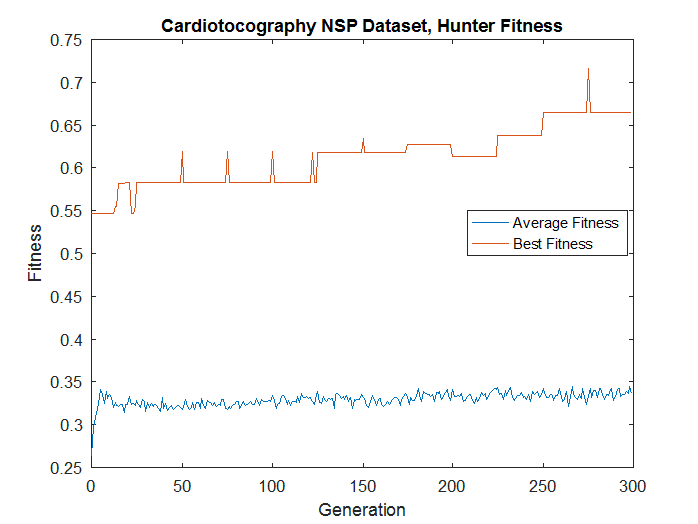
\includegraphics[width=0.7\linewidth]{figures/png/fitnessCardioNSPHunter}
	\caption[Hunter Population Growth, CardioNSP]{This figure demonstrates Hunter fitness, average and best, over the lifespan of a trial, in this case 300 generations. Where there seems to be lacking monotonicity is actually the result of validation fitness, which has the best Hunters seemingly scoring much better on the testing set.}
	\label{fig:fitnesscardionsphunter}
	
	\includegraphics[width=0.7\linewidth]{figures/png/fitnessCardioNSPMcNB}
	\caption[Multiclass Na\"ive Bayes Optimizer Growth, CardioNSP]{
	Population fitness of the McNB Optimizer on the CardioNSP dataset.  This overall shape is typical of most Optimizers.}
	
\end{figure}

It is clear that theoretically based algorithms are better at solving problems than trying to co-opt a GA to do it on its own.  
As for whether we should use McNB or CTree, the answer is clear: neither.  We've already written far better performing algorithms elsewhere, including aggregate trees and support vector machine optimizers.  The purpose of those algorithms was to give Hunters competition that wouldn't completely outclass them, and they failed in that regard.  This is at least partially because Na\"ive Bayes is such a robust first pass, and there are good reasons to use it in ensemble methods because it does such a good job extracting signal from messy data.  Further, it does a decent job differentiating classes with few samples.\\
The most surprising performance was from CTree- while we have used trees in aggregate before, they performed far better alone than expected, in some regards holding their own up against Na\"ive Bayes, though mostly in terms of overall accuracy and only if we're being accommodating.  Still, their performance was better than we would have expected going into the project.\\
Hunters performed poorly.  There might be some way of improving their performance, which we've noted as we've gone through the document.  However, there should be a case made that such an endeavor is worthwhile, and one would need significant data contradicting this paper to say that there remains a compelling reason to do so.  When we began this project, we believed that they had a decent chance to at least hold their own with our methods.  This has been proven to be false across numerous comparisons.  Further, we ``cheated" on behalf of the Hunter, giving it vast additional resources, time, and modified starting conditions.  We gave it every advantage, and it failed to deliver.  The evidence is not conclusive for genetic algorithms in general, but this GA specifically is vastly inferior to even modest hybrid classification methods and should be retired.  